In this section the five methods we have explained will be compared in term of performances, in addition also two other methods which have been explored during the lectures will be considered, SimCLR \cite{chen2020simple} and BYOL \cite{grill2020bootstrap}. As we already said in the previous sections, the way in which we evaluate SSL methods is by evaluating how downstream tasks perform after the SSL phase. Of course the evaluation on the downstream task might depends by many factors: the chosen dataset, the type of the architecture, the network used for the encoding, the hyper-parameters used for the methods and so on. In this section I tried to use the results taken from the papers of the considered methods, from survey \cite{technologies9010002} and from this paper \cite{ericsson2021well}. In order to have a fair comparison I tried to collect results when the methods have been compared with the same encoder, and I compared the methods on different datasets.

\noindent In table \ref{tab:imagenet-top1-5-acc-comp} we report the top-1 and top-5 accuracy of the considered methods when tested for classification on the ImageNet dataset and also the performances of a supervised model trained directly without SSL. All the methods uses as feature extractor a ResNet50 and the fine-tuning the SSL model is frozen and we train a linear classifier. SWAV and BYOL are by far the two best performing models even if they do not reach the top-1 accuracy of the supervised model.

\begin{table}[H]
	\centering
	\begin{tabular}{|l|l|cc|}
		\hline
		\multicolumn{1}{|c|}{\textbf{Method}} & \textbf{Architecture} & \multicolumn{2}{c|}{\textbf{ImageNet}} \\
		\multicolumn{1}{|c|}{} &  & Top1 & Top5 \\
		\hline
		Supervised & ResNet50 & 76.5 & - \\
		\hline
		PIRL & ResNet50 & 63.6 & - \\
		CPCv2 & ResNet50 & 63.8 & 85.3 \\
		CMC & ResNet50  & 66.2 & 87 \\
		SimCLR & ResNet50 & 69.3 & 89.0 \\
		MoCov2 & ResNet50 & 71.1 & - \\
		BYOL & ResNet50  & 74.3 & 91.6 \\ 
		SwAV & ResNet50 & 75.3 & - \\
		\hline
\end{tabular}
	\caption{Accuracy of the SSL methods using linear probing for fine-tuning}
	\label{tab:imagenet-top1-5-acc-comp}
\end{table}


Table \ref{tab:imagenet-1-perc-semisup} shows the performances of the methods in semi-supervised learning scenario. Basically after having performed the SSL models before evaluating the on the classification task on ImageNet we first fine-tune the model using in one case the 1\% and in the other case the 10\% of the data. We report also same version of the same model with different encoder sizes. If we only look at the models that use the ResNet50 the raking of the model is the same that we obtained in the case of the linear probing. Here we can also se that the network used for the encoding can impact the performances CPCv2 reaches an higher top-5 accuracy than SWAV and BYOL with a ResNet50.

\begin{table}[H]
	\centering
	\begin{tabular}{|l|l|cc|cc|}
		\hline
		\multicolumn{1}{|c|}{\textbf{Method}} & \textbf{Architecture} & \multicolumn{2}{c|}{\textbf{ImageNet 1\%}} & \multicolumn{2}{c|}{\textbf{ImageNet 10\%}} \\
		\multicolumn{1}{|c|}{} &  & Top1 & Top5 & Top1 & Top5  \\
		\hline
		Supervised & ResNet50 & 25.4 & 48.4 & 56.4 & 80.4 \\
		PIRL & ResNet50 & 30.7 & 57.2  & 60.4 & 83.8 \\
		SimCLR & ResNet50 & 48.3 & 75.5  & 65.6 & 87.8 \\
		BYOL & ResNet50  & 53.2 & 78.4  & 68.8 & 89.0 \\ 
		SwAV & ResNet50 & 53.9 & 78.5  & 70.2 & 89.9 \\
		CPCv2 & ResNet161 & - & 77.9 & - & 91.2 \\
		SimCLR & ResNet50 (4$\times$) & 63.0 & 85.8 & 74.4 & 92.6 \\
		BYOL & ResNet50 (2$\times$) & 71.2 & 89.5 & 77.7 & 93.7 \\
		\hline
	\end{tabular}
	\caption{Semi-supervised learning accuracy}
	\label{tab:imagenet-1-perc-semisup}
\end{table}

In tables \ref{tab:classification-multi-dataset-linear} and \ref{tab:classification-multi-dataset-finetune} we report the accuracy for image classification task of the considered methods on multiple datasets using the same encoder for every method (a ResNet50). In table \ref{tab:classification-multi-dataset-linear} the pre-trained feature extractor is kept frozen and the classification is performed using multinomial logistic regression, while in table \ref{tab:classification-multi-dataset-finetune} the whole architecture is fine-tuned with SGD. In the right-most column we report the average accuracy across all the datasets. 
\begin{table}[H]
	\centering
	\scalebox{0.6}{
	\begin{tabular}{l|cccccccccccc|c|}
		\cline{2-14}
		& \multicolumn{1}{c|}{\textbf{Imagenet}} & \multicolumn{1}{c|}{\textbf{Aircraft}} & \multicolumn{1}{c|}{\textbf{Calthech101}} & \multicolumn{1}{c|}{\textbf{Cars}} & \multicolumn{1}{c|}{\textbf{CIFAR10}} & \multicolumn{1}{c|}{\textbf{CIFAR100}} & \multicolumn{1}{c|}{\textbf{DTD}} & \multicolumn{1}{c|}{\textbf{Flowers}} & \multicolumn{1}{c|}{\textbf{Food}} & \multicolumn{1}{c|}{\textbf{Pets}} & \multicolumn{1}{c|}{\textbf{SUN387}} & \multicolumn{1}{c|}{\textbf{VOC2007}} & \multicolumn{1}{c|}{\textbf{Average}} \\ \hline
		\multicolumn{1}{|l|}{Supervised} & 77.20 & 43.59 & 90.18 & 44.92 & 91.42 & 73.90 & 72.23 & 89.93 & 64.49 & 91.45 & 60.49 & 83.60 & 73.75 \\ \hline
		\multicolumn{1}{|l|}{PIRL} & 61.70 & 37.08 & 74.48 & 28.72 & 82.53 & 61.26 & 68.99 & 83.60 & 64.65 & 71.36 & 53.89 & 76.61 & 63.92 \\ \cline{1-1}
		\multicolumn{1}{|l|}{SimCLR} & 69.30 & 44.90 & 90.05 & 43.73 & 91.18 & 72.73 & 74.20 & 90.87 & 67.47 & 83.33 & 59.21 & 80.77 & 72.59 \\ \cline{1-1}
		\multicolumn{1}{|l|}{MoCo-v2} & 71.10 & 41.79 & 87.92 & 39.31 & 92.28 & 74.90 & 73.88 & 90.07 & 68.95 & 83.30 & 60.32 & 82.69 & 72.31 \\ \cline{1-1}
		\multicolumn{1}{|l|}{BYOL} & 74.30 & 53.87 & 91.46 & 56.40 & 93.26 & 77.86 & 76.91 & 94.50 & 73.01 & 89.10 & 59.99 & 81.14 & 77.05 \\ \cline{1-1}
		\multicolumn{1}{|l|}{SWAV} & 75.30 & 54.04 & 90.84 & 54.06 & 93.99 & 79.58 & 77.02 & 94.62 & 76.62 & 87.60 & 65.58 & 83.68 & 77.97 \\ \hline
	\end{tabular}
	}
	\caption{Result after fine-tuning on 1\% of the data of ImageNet}
	\label{tab:classification-multi-dataset-linear}
\end{table}

\begin{table}[H]
	\centering
	\scalebox{0.6}{
	\begin{tabular}{l|ccccccccccc|c|}
		\cline{2-13}
		& \multicolumn{1}{c|}{\textbf{Aircraft}} & \multicolumn{1}{c|}{\textbf{Calthech101}} & \multicolumn{1}{c|}{\textbf{Cars}} & \multicolumn{1}{c|}{\textbf{CIFAR10}} & \multicolumn{1}{c|}{\textbf{CIFAR100}} & \multicolumn{1}{c|}{\textbf{DTD}} & \multicolumn{1}{c|}{\textbf{Flowers}} & \multicolumn{1}{c|}{\textbf{Food}} & \multicolumn{1}{c|}{\textbf{Pets}} & \multicolumn{1}{c|}{\textbf{SUN387}} & \multicolumn{1}{c|}{\textbf{VOC2007}} & \multicolumn{1}{c|}{\textbf{Average}} \\ \hline
		\multicolumn{1}{|l|}{Supervised} & 83.50 & 91.01 & 82.61 & 96.39 & 82.91 & 73.30 & 95.50 & 84.60 & 82.42 & 63.56 & 84.76 & 84.60 \\ \cline{1-1}
		\multicolumn{1}{|l|}{PIRL} & 72.68 & 70.83 & 61.02 & 92.3 & 66.48 & 64.26 & 89.81 & 74.96 & 76.26 & 50.38 & 69.90 & 71.71 \\ \cline{1-1}
		\multicolumn{1}{|l|}{SimCLR} & 81.06 & 90.35 & 83.78 & 97.07 & 84.53 & 71.54 & 93.75 & 82.40 & 84.10 & 63.31 & 82.58 & 83.13 \\ \cline{1-1}
		\multicolumn{1}{|l|}{MoCo-v2} & 78.87 & 84.38 & 75.20 & 96.45 & 71.33 & 69.47 & 94.35 & 76.78 & 78.80 & 55.77 & 71.71 & 77.74 \\ \cline{1-1}
		\multicolumn{1}{|l|}{BYOL} & 79.45 & 89.40 & 84.60 & 97.01 & 83.95 & 73.62 & 94.48 & 85.54 & 89.62 & 63.96 & 82.70 & 84.03 \\ \cline{1-1}
		\multicolumn{1}{|l|}{SWAV} & 83.08 & 89.85 & 86.76 & 96.78 & 84.37 & 75.16 & 95.46 & 87.22 & 89.05 & 66.24 & 84.66 & 85.33 \\ \hline
	\end{tabular}
	}
	\caption{Result after fine-tuning on 1\% of the data of ImageNet}
	\label{tab:classification-multi-dataset-finetune}
\end{table}
Even in these experiments SWAV performs slightly better than BYOL (even if in not all the datasets). SimCLR and MoCo have similar performances while PIRL performs significantly worse.

In table \ref{tab:object-detection-swav} we report the results of the method using object detection as downstream task on the VOC dataset. The network used for the encoding is a Faster R-CNN FPN.
\begin{table}[H]
	\centering
	\begin{tabular}{l|ccc|ccc|}
		\cline{2-7}
		& \multicolumn{3}{c|}{VOC (frozen)} & \multicolumn{3}{c|}{VOC (finetune)} \\ \cline{2-7} 
		& \multicolumn{1}{c}{AP} & \multicolumn{1}{c}{AP50} & \multicolumn{1}{c|}{AP75} & \multicolumn{1}{c}{AP} & \multicolumn{1}{c}{AP50} & \multicolumn{1}{c|}{AP75} \\ \hline
		\multicolumn{1}{|l|}{Supervised} & 51.99 & 81.53 & 56.21 & 53.26 & 81.51 & 59.07 \\ \hline
		\multicolumn{1}{|l|}{PIRL} & 49.54 & 77.26 & 52.79 & 45.08 & 72.50 & 47.80 \\ \cline{1-1}
		\multicolumn{1}{|l|}{SimCLR} & 51.94 & 81.19 & 56.49 & 52.19 & 81.36 & 56.92 \\ \cline{1-1}
		\multicolumn{1}{|l|}{MoCo-v2} & 54.22 & 81.86 & 59.97 & 44.74 & 72.82 & 47.01 \\ \cline{1-1}
		\multicolumn{1}{|l|}{BYOL} & 53.32 & 82.01 & 58.37 & 54.91 & 82.57 & 60.82 \\ \cline{1-1}
		\multicolumn{1}{|l|}{SWAV} & 50.68 & 80.82 & 54.11 & 52.07 & 81.50 & 56.03 \\ 
		\hline
	\end{tabular}
	\caption{Result after fine-tuning on 1\% of the data of ImageNet}
	\label{tab:object-detection-swav}
\end{table}
In this case is BYOL that performs slightly better than SWAV.

\begin{comment}
\begin{table}[H]
	\centering
	\begin{tabular}{l|ccc||ccc|}
		\cline{2-7}
		\multicolumn{1}{c|}{\textbf{}} & \multicolumn{3}{c||}{\textbf{Linear classification}} & \multicolumn{3}{c|}{\textbf{Object detection}} \\ \cline{2-7} 
		& \multicolumn{1}{l|}{Places205} & \multicolumn{1}{l|}{VOC07} & \multicolumn{1}{l||}{iNat18} & \multicolumn{1}{l|}{VOC07+12} & \multicolumn{1}{l|}{COCO} & \multicolumn{1}{l|}{COCO} \\ \hline
		\multicolumn{1}{|l|}{Supervised} & \multicolumn{1}{c|}{53.2} & \multicolumn{1}{c|}{87.5} & 46.7 & \multicolumn{1}{c|}{81.3} & \multicolumn{1}{c|}{39.7} & 40.8 \\ \hline
		\multicolumn{1}{|l|}{PIRL} & \multicolumn{1}{c|}{49.8} & \multicolumn{1}{c|}{81.1} & 34.1 & \multicolumn{1}{c|}{80.7} & \multicolumn{1}{c|}{-} & - \\ \hline
		\multicolumn{1}{|l|}{SimCLR} & \multicolumn{1}{c|}{53.3} & \multicolumn{1}{c|}{86.4} & 36.2 & \multicolumn{1}{c|}{-} & \multicolumn{1}{c|}{-} & - \\ \hline
		\multicolumn{1}{|l|}{MoCov2} & \multicolumn{1}{c|}{52.9} & \multicolumn{1}{c|}{87.1} & 38.9 & \multicolumn{1}{c|}{82.5} & \multicolumn{1}{c|}{39.8} & 42.0 \\ \hline
		\multicolumn{1}{|l|}{SWAV} & \multicolumn{1}{c|}{56.7} & \multicolumn{1}{c|}{88.9} & 48.6 & \multicolumn{1}{c|}{82.6} & \multicolumn{1}{c|}{41.6} & 42.1 \\ \hline
	\end{tabular}
	\caption{Result after fine-tuning on 1\% of the data of ImageNet}
	\label{tab:object-detection-swav}
\end{table}
\end{comment}

\begin{comment}
\begin{table}[H]
	\centering
	\begin{tabular}{l|ccc||ccc||ccc|}
		\cline{2-10}
		& \multicolumn{3}{c||}{\textbf{VOC 07+12 detection}} & \multicolumn{3}{c||}{\textbf{COCO detection}} & \multicolumn{3}{c|}{\textbf{COCO instance seg.}} \\ \hline
		\multicolumn{1}{|l||}{\textbf{Method}} & \multicolumn{1}{c|}{AP\_50} & \multicolumn{1}{c|}{AP} & AP$_{75}$ & \multicolumn{1}{c|}{AP\_50} & \multicolumn{1}{c|}{AP} & AP\_75 & \multicolumn{1}{c|}{AP\_50} & \multicolumn{1}{c|}{AP} & AP\_75 \\ \hline
		\multicolumn{1}{|l||}{MoCov2} & \multicolumn{1}{c|}{82.7} & \multicolumn{1}{c|}{57.9} & 64.5 & \multicolumn{1}{c|}{61.0} & \multicolumn{1}{c|}{41.1} & 44.8 & \multicolumn{1}{c|}{57.7} & \multicolumn{1}{c|}{35.8} & 38.4 \\ \hline
		\multicolumn{1}{|l||}{BYOL} & \multicolumn{1}{c|}{82.7} & \multicolumn{1}{c|}{56.7} & 63.0 & \multicolumn{1}{c|}{61.1} & \multicolumn{1}{c|}{40.9} & 44.5 & \multicolumn{1}{c|}{57.6} & \multicolumn{1}{c|}{35.5} & 37.8 \\ \hline
		\multicolumn{1}{|l||}{SWAV} & \multicolumn{1}{c|}{82.3} & \multicolumn{1}{c|}{55.6} & 61.9 & \multicolumn{1}{c|}{61.4} & \multicolumn{1}{c|}{40.7} & 43.7 & \multicolumn{1}{c|}{57.6} & \multicolumn{1}{c|}{35.4} & 37.4 \\ \hline
	\end{tabular}
	\caption{Result after fine-tuning on 1\% of the data of ImageNet}
	\label{tab:object-detection-comp}
\end{table}
\end{comment}

\begin{comment}
\begin{table}[H]
	\centering
	\begin{tabular}{|l|l|c|c|}
		\hline
		\multicolumn{1}{|c|}{Method} & \multicolumn{1}{c|}{Architecture} & AP\_50 & mIoU \\ \hline
		Supervised & ResNet50 & 74.4 & 74.4 \\ \hline
		MoCo & ResNet50 & 74.9 & 72.5 \\ \hline
		CPC & ResNet161 & 76.6 & - \\ \hline
		SimCLR & ResNet50 & 75.2 & 75.2 \\ \hline
		BYOL & ResNet50 & 77.5 & 76.3 \\ \hline
	\end{tabular}
	\caption{Result after fine-tuning on 1\% of the data of ImageNet}
	\label{tab:object-detection-byol}
\end{table}

\begin{comment}
Figure \ref{fig:imagenet-top1-acc-comp} shows the accuracy of SSL methods with encoders of different parameters sizes in image classification for ImageNet, and it highlights that the number of parameters of the model is important to get high performances. For instances CPCv2 with a large encoder performs better that MoCo and SimCLR with a smaller encoder.
\begin{figure}[H]
	\centering
	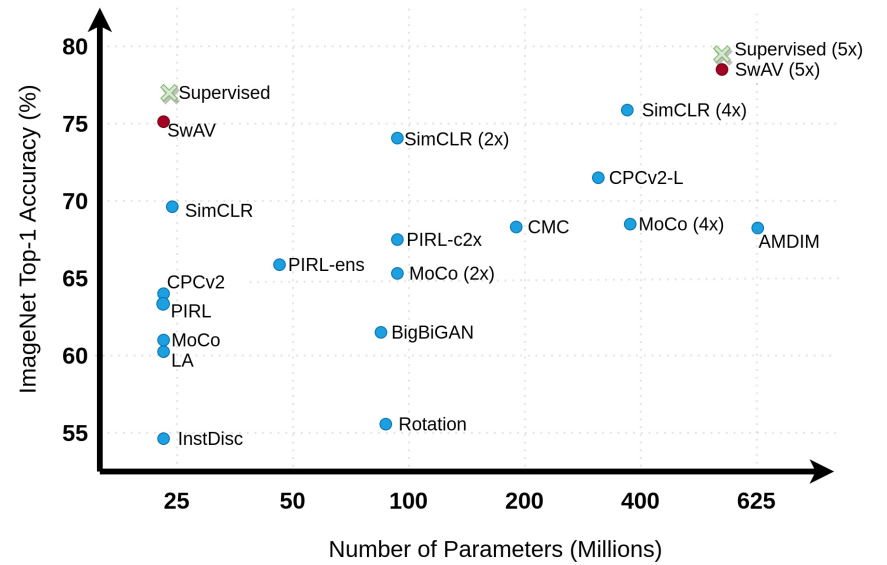
\includegraphics[width=10cm]{./images/imagenet-top1-acc-comp.png}
	\caption{Top-1 classification accuracy different contrastive learning methods with the number of parameters of the models}
	\label{fig:imagenet-top1-acc-comp}
\end{figure}
\end{comment}